\chapter{Adquisión de conocimiento}

La adquisición y educción del conocimiento constituye una de las fases más importantes del desarrollo de este tipo de sistemas. En esta etapa es donde el Ingeniero del Conocimiento interactúa con el experto para obtener la información sobre la solución de los problemas, así como las estrategias utilizadas para la obtención de cada solución. Además de consultar con el experto, también se adquiere conocimiento de otras fuentes como libros, tratados, estudios, etc. Este proceso supone el ``cuello de botella'' del desarrollo.
 
Esta tarea no es un paso concreto en la metodología de desarrollo, sino que se va produciendo en paralelo al resto de etapas de construcción del sistema.

El proceso de adquisión de conocimiento se ha llevado a cabo en tres fases: 

\begin{itemize}
	\item Extracción de conocimientos
	\item Educción de conocimientos
	\item Estructuración de conocimientos
\end{itemize}
 
Para llevar a cabo estas tareas, he consultado a los expertos Alberto José Moreno Montes e Isabel Salado Ortega, ambos músicos titulados.  

\section{Extracción de conocimientos}

En la realización de esta tarea, se pretende aprender sobre el dominio tanto como sea posible antes de comenzar las sesiones con los expertos para facilitar la educción de conocimientos. 

Al haber estudiado música en el conservatorio hace algunos años, esta fase supuso más bien un proceso de recordar que de aprender. No obstante, al ser un dominio tan extenso, es necesario consultar la documentación adecuada y más útil para la aplicación a nuestro problema. Por este motivo, pregunté a ambos expertos, Alberto e Isabel, sobre el material más importante a consultar, incluyendo libros, manuales y tratados. Las dos fuentes más relevantes y de las cuáles se extrajo la mayoría de conocimientos previos fueron el \textit{Tratado de Armonía}, vólumenes I y II,de Joaquín Zamacois \cite{ZAMACOIS1, ZAMACOIS2} y \textit{Armonía} por Walter Piston \cite{PISTON}. Ambos se incluyen, junto con el resto de fuentes, en las referencias bibliográficas. 

De estos libros se determinaron la mayoría de definiciones y conceptos generales sobre lenguaje musical y armonía.

\section{Educción de conocimientos}

Gracias a los conocimientos adquiridos en la fase anterior, realizamos una serie de entrevistas estructuradas con los expertos. En estas entrevistas se formularon cuestiones concretas y previamente planificadas con el fin de educir conocimiento de una forma más eficiente. Nos centramos en definir conceptos específicos y procedimientos necesarios a la hora de analizar partituras, haciendo especial énfasis en el análisis melódico, el cual tiende a ser más delicado de realizar y con un componente subjetivo más fuerte.

La mayor dificultad de este proceso radicó en la cantidad de situaciones excepcionales que pueden darse y de la subjetividad que viene adherida a cualquier arte. Por ejemplo, las excepciones a la falta de \textit{quintas paralelas}. Las \textit{quintas paralelas} son una de las faltas más graves, dado que al darse se produce una sonoridad más dura y arcaica. Sin embargo, éstas pueden permitirse si la segunda quinta que se forma es una quinta disminuida, salvo que ésta se forme con el bajo o en voces extremas, en cuyo caso se considerará falta.

Como podemos observar en este ejemplo, las reglas armónicas no son directrices sencillas de llevar a cabo o entender fácilmente. Con el fin de poder comprenderlas empleé con Alberto e Isabel lo que denominamos ``incidentes críticos''. 

\subsection{Incidentes críticos}
 
Con la técnica de ``incidentes críticos'', ambos expertos me describieron los casos excepcionales mencionados anterioremente y algunas de las dificultades más relevantes a la hora de realizar un análisis armónico y/o melódico. 

Me explicaron todas las posibles excepciones para cada regla, ejemplificándome cada una de las situaciones. 

En el caso de los problemas derivados por la subjetividad a la hora de analizar las melodías de un coral, Alberto sugirió ceñirse lo más posible al estilo de los corales compuestos durante la época barroca, ya que las restricciones a la hora de componer eran más fuertes y estaban mejor delimitadas.  

\section{Estructuración de conocimientos} 

Una vez hemos finalizado la extracción y la educción de conocimientos pasamos a analizar, organizar y estructurar todos los conocimientos obtenidos para crear nuestra base de conocimiento.

En un primer paso, constrastamos toda la información que hemos adquirido junto con los requisitos del sistema para filtrar qué conocimientos son los necesarios y útiles para poder llevar a cabo los distintos análisis en el coral. Los tipos de análisis son independientes entre sí, por lo que se hizo una filtración de información para cada uno de ellos. Aunque el tener distintos análisis sobre la partitura podía suponer una dificultad para este proceso de selección, el hecho de ser independientes supuso una gran ventanja, facilitándolo en gran medida. 

A continuación, organizamos y estructuramos el conocimiento diviéndolo en \textit{hechos} y \textit{reglas}. 

\begin{itemize}

	\item Los \textit{hechos} serán asertados en el sistema. Para definir la mayoría de estos hechos se hará uso de estructuras ``\texttt{templates}'' o plantillas.

	\bigskip

		\begin{lstlisting}

			(intervalo (distancia d) (tipo t) (nota1 n1) (nota2 n2))

		\end{lstlisting}

	\bigskip

	\item Las \textit{reglas} definirán los requisitos funcionales del sistema en forma de estructuras \textit{si <<antecedente>> entonces <<consecuente>>}. 

	\bigskip

		\begin{lstlisting}

			if intervalo.distancia = 2 then intervalo.tipo = disonante

		\end{lstlisting}

	\bigskip

\end{itemize} 

Este conjunto de hechos y reglas constituirá la base de conocimiento del sistema experto. Estas reglas utilizarán los hechos almacenados en la base de conocimiento, junto con los hechos calculados a partir de los datos de entrada, para deducir nuevos hechos y conocimientos que permitan obtener conclusiones finales y así obtener resultados.

\subsection{Hechos}

Los hechos del sistema se dividen en tres tipos:

\begin{itemize}

	\item \textbf{Hechos asertados}: son los hechos que constituyen la base de conocimiento ``inicial'' del sistema. Estos hechos constituyen todo el conocimiento necesario ,referido principalmente a conceptos, para poder analizar una partitura. 

	\item \textbf{Hechos calculados}: son los hechos que extraemos directamente de la partitura, es decir, las notas que la componen con sus alteraciones, su altura y su duración.

	\item \textbf{Hechos deducidos}: son los hechos que el sistema deduce aplicando las reglas a los hechos asertados y calculados. También puede deducir hechos a partir de hechos previamente deducidos que sea utilizados por las reglas.

\end{itemize}

\bigskip

Los hechos asertados están referidos a los siguientes conceptos:

\begin{itemize}

	\item \textit{Tonalidades}: todas las posibles tonalidades existentes indicando el nombre de la tonalidad, el modo, las alteraciones que tienen en su armadura y la sensible.

	\begin{lstlisting}

		(tonalidad (nombre D) (tipo mayor) (armadura 2s) (sensible Cs))

	\end{lstlisting}

	Las tonalidades las usaremos para poder determinar qué tipo de alteraciones tienen las notas de la partitura por defecto y cuáles serían alteraciones accidentales. También nos indican la sensible de la tonalidad, la cuál usaremos para comprobar varios errrores.

	\bigskip

	\item \textit{Escalas}: todas las escalas mayores y menores asociadas a cada tonalidad, indicando el nombre de la escala y las notas (grados) que la componen. 

	\begin{lstlisting}

		(escala (nombre D) (tipo mayor) (grado_I G) (grado_II A) (grado_III B) (grado_IV C) (grado_V D) (grado_VI E) (grado_VII Fs))

	\end{lstlisting}

	A partir de la escala podemos deducir todos los acordes fundamentales de la tonalidad. Con ellos realizaremos el análisis armónico comprobando acordes incompletos, sucesiones erróneas, etc.

	\bigskip

	\item \textit{Intervalos}: todos los tipos de intervalos desde segundas menores hasta octavas justas desde cada una de las posibles notas. Indicamos la distancia, el tipo y las dos notas que lo forman.

	\begin{lstlisting}

		(intervalo (distancia 3) (tipo mayor) (nota1 G) (nota2 B))

	\end{lstlisting}

	Necesitamos conocer todos los intervalos posibles para poder evaluar saltos y contrapunto en las melodías, así como movimientos armónicos entre las voces, como las quintas paralelas u octavas entre otras faltas.

	\bigskip

	\item \textit{Acordes}: todos los acordes de cada uno de los grados de cada tonalidad. Los acordes pueden ser de tríada (formados por tres notas) o cuatríada (formados por cuatro notas), por lo que diferenciamos ambos tipos. Indicamos el grado de la escala a partir de la cuál se forma el acorde, el nombre y el modo de la tonalidad a la que pertenece y las notas que lo componen: fundamental, tercera y quinta en el caso de acordes de tríada y fundamental, tercera, quinta y séptima en el caso de acordes de cuatríada.

	\begin{lstlisting}

		(acorde_3 (grado I) (nombre_tonalidad C) (modo_tonalidad mayor) (fundamental C) (tercera E) (quinta G))

	\end{lstlisting}

	\begin{lstlisting}

		(acorde_4 (grado V) (nombre_tonalidad C) (modo_tonalidad mayor) (fundamental G) (tercera B) (quinta D) (septima F))

	\end{lstlisting}

	Los acordes los utilizaremos para poder realizar el análisis armónico.

	\bigskip

	\item \textit{Sucesiones lógicas}: lista de sucesiones permitidas entre acordes según las normas de la armonía tradiciones. Se indican los dos grados que componen una sucesión lógica.

	\begin{lstlisting}

		(sucesion_logica (grado1 V) (grado2 I))

	\end{lstlisting} 

	Esto nos permite analizar la coherencia armónica de la obra, es decir, que la estructura armónica sobre la que se construye el coral sea correcta y tenga una buena sonoridad.

\end{itemize}

\bigskip

Los hechos calculados del sistema son aquellos que extraemos a partir de la información contenida en la partitura.

\begin{itemize}

	\item Tonalidad: se extrae la tonalidad de la obra para poder determinar sobre qué escala tenemos que trabajar y qué acordes son los que vamos a analizar.

	\item Compás: se extrae el compás para poder localizar los errores.

	\item Notas: se extrae la información sobre las notas de la partitura. Dependiendo de si se va a realizar un análisis melódico o armónico extraeremos dos listas distintas de notas.

	\item Movimientos: se extrae también información sobre los movimientos de las notas para poder analizar tanto errores armónicos como melódicos.

\end{itemize}

\bigskip

Toda la información referida a estos hechos se explicará con más detalle en el apartado de la implementación.

\bigskip

Poŕ último, los hechos deducidos serán los que irá asertando el sistema tras aplicar reglas y utilizará para ir deduciendo nuevos hechos hasta llegar a las conclusiones finales, que en este caso serán la existencia o no de errores y faltas.

\subsection{Reglas}

Las reglas del sistema coinciden prácticamente con los requisitos funcionales descritos en el capítulo anterior, aunque para poder implementar algunas de estas reglas ha sido necesario añadir reglas auxiliares.

\begin{itemize}

	\item \textit{Reglas para cargar los hechos iniciales}: debido a varios problemas con la implementación, que se comentarán en el capítulo 5, los hechos asertados comentados en el apartado anterior serán asertados a partir de unas reglas que los cargarán en la memoria de trabajo. 

	\bigskip

	\item \textit{Reglas para la lectura de los datos extraídos de la partitura}: a continuación cargamos los hechos calculados. Estos son la información referida a las notas de la partitura, que ha sido previamente procesada para facilitar la aserción de estos hechos.
 
	\bigskip

	\item \textit{Reglas para detección de quintas}: este conjunto de reglas se encarga de detectar errores de quintas paralelas y quintas directas, teniendo en cuenta posibles casos excepcionales.

	\bigskip

	\item \textit{Reglas para detección de octavas}: detectan errores de octavas paralelas y octavas directas, comprobando posibles casos excepcionales.

	\bigskip

	\item \textit{Reglas para detección de tritonos armónicos}: comprueban si se da alguna el intervalo de cuarta aumentada entre dos voces, teniendo en cuenta la excepción de si está o no preparado.

	\bigskip

	\item \textit{Regla para comprobar la dulpicación de sensible}: comprueba que la sensible no se encuentre duplicada en dos voces bajo ninguna circunstancia.

	\bigskip

	\item \textit{Regla para comprobar la resolución de sensible}: esta regla comprueba que la sensible resuelva correctamente en la tónica de la tonalidad.

	\bigskip

	\item \textit{Regla para comprobar la resolución de séptima}: al igual que en el caso de la sensible, se comprueba que la séptima también resuelva correctamente, sin tener en cuenta ninguna resolución excepcional.

	\bigskip

	\item \textit{Reglas para comprobar tritonos y segundas aumentadas melódicas}: estas reglas comprueban que no se produzcan este tipo de intervalos en la melodía de ninguna voz.

	\bigskip

	\item \textit{Reglas para comprobar el contrapunto en voces extremas}: este conjunto de reglas analiza los movimientos de las melodías de la soprano y el bajo para comprobar que predomina el movimiento contrario u oblicuo sobre el movimiento directo entre las voces.

	\bigskip

	\item \textit{Reglas para comprobar el contrapunto del salto}: este conjunto de reglas realiza una función similar al contrapunto de voces extremas, pero se centra en cada línea melódica. Se comprueba que no se den saltos que puedan provocar disonancias.

	\bigskip

	\item \textit{Reglas para comprobar las líneas melódicas}: estas reglas analizan los movimientos de las voces respecto a si se hacen demasiados saltos grandes o predomina el movimiento por grado conjunto en las melodías. Con esto podemos determinar si una melodía está bien construida o por el contrario no tiene coherencia melódica.

	\bigskip

	\item \textit{Reglas para analizar acordes}: se analizan armónicamente el coral determinando su estructura armónica. Se consideran tanto acordes de tríada como acordes con séptima teniendo en cuenta sus posibles inversiones.

	\bigskip

	\item \textit{Reglas para analizar la lógica tonal}: a partir del análisis previo de los acordes, se comprueba que las sucesiones de éstos sean correctas y sigan patrones armónicos tradicionales.

	\bigskip

	\item \textit{Reglas para comprobar los acordes}: este conjunto de reglas comprueba que todos los acordes estén completos, es decir, que no falte ninguna de las notas que lo componen por hacer una mala duplicación de las notas en las voces. 

	\bigskip

	\item \textit{Reglas para mostrar los errores}: una vez detectados todos los errores con las reglas anteriores, implementamos una serie de reglas para poder mostrar los errores al usuario. Cada error se muestra debidamente explicado y localizado en la partitura.

\end{itemize}

\bigskip

\subsection{Estructura}

En total el sistema está compuesto por 873 hechos iniciales, previamente asertados, y 174 reglas. Hay que tener en cuenta que estos hechos iniciales son los hechos asertados, sin tener en cuenta todos los hechos que serán extraídos de la partitura. Dependiendo de la longitud del coral, se asertarán más o menos hechos calculados. Podemos estimar la cantidad de hechos calculados referidos a las notas de la siguiente manera:

\begin{itemize}

	\item Si el compás es binario:
		$$hechos\_calculados\_notas = n^{\circ}\ de\ partes\ del\ compas \times 16 \times n^{\circ}\ de\ compases$$

	\item Si el compás es ternario:
		$$hechos\_calculados\_notas = n^{\circ}\ de\ partes\ del\ compas \times 8 \times n^{\circ}\ de\ compases$$

\end{itemize}

\bigskip

Para hacernos una idea más exacta, si nuestro coral tiene 24 compases y un compás \lilyTimeSignature{4}{4} (compás binario de cuatro partes) en total tendríamos de 1536 hechos referidos únicamente a las notas. Tenemos que tener en cuenta que estos serían utilizados únicamente para realizar el análisis armónico. Para realizar el análisis melódico necesitamos el número de notas de cada voz, que dependerá del coral y no podemos conocer su número a priori. Además, tenemos otra serie de hechos calculados como los movimientos de las notas, que serán iguales a la cantidad de notas para el análisis melódico.

Esto significa que para analizar de manera completa un coral de la misma longitud y compás que el del ejemplo anterior y suponiendo que sea un coral sencillo sin demasiadas notas, vamos a suponer tres notas por compás en cada voz, contaríamos con cerca de 3000 hechos inicales.

Para facilitar la implementación y hacerlo más usable, como se ha comentado anteriormente, el sistema estará formado por varios módulos. A continuación se muestra un listado de los módulos indicando los hechos y reglas que los componen y el número de estos, sin tener en cuenta el número de hechos calculados que dependerán de la partitura:

\begin{itemize}

	\item \textbf{Módulo 1}: 408 hechos y 42 reglas.

	\begin{itemize}

		\item Hechos asertados:

			\begin{itemize}

				\item Tonalidades

				\item Intervalos

			\end{itemize}

		\item Hechos calculados:

			\begin{itemize}

				\item Tonalidad de la obra

				\item Compás

				\item Lista de notas de las voces para análisis armónico

				\item Lista de los movimientos de las melodías

			\end{itemize}

		\item Reglas:

			\begin{itemize}

				\item Reglas para cargar hechos iniciales

				\item Reglas para cargar hechos calculados

				\item Reglas para errores de quintas

				\item Reglas para errores de octavas

				\item Reglas para tritonos armónicos

				\item Regla para duplicación de sensible

				\item Reglas para mostrar errores

			\end{itemize}

	\end{itemize}

	\bigskip

	\item \textbf{Módulo 2}: 858 hechos y 82 reglas.

	\begin{itemize}

		\item Hechos asertados:

			\begin{itemize}

				\item Tonalidades

				\item Intervalos

				\item Escalas

				\item Acordes

			\end{itemize}

		\item Hechos calculados:

			\begin{itemize}

				\item Tonalidad de la obra

				\item Compás

				\item Lista de notas de las voces

				\item Lista de los movimientos de las melodías

			\end{itemize}

		\item Reglas:

			\begin{itemize}

				\item Reglas para cargar hechos iniciales

				\item Reglas para cargar hechos calculados

				\item Regla para resolución de sensible

				\item Regla para resolución de séptima

				\item Reglas para intervalos disonantes melódicos

				\item Reglas para contrapunto en voces extremas

				\item Reglas para contrapunto del salto

				\item Reglas para comprobar líneas melódicas

				\item Reglas para mostrar errores

			\end{itemize}
			
	\end{itemize}

	\bigskip

	\item \textbf{Módulo 3}: 875 hechos y 50 reglas.

	\begin{itemize}

		\item Hechos asertados:

			\begin{itemize}

				\item Tonalidades

				\item Intervalos

				\item Escalas

				\item Acordes

				\item Lógica tonal

			\end{itemize}

		\item Hechos calculados:

			\begin{itemize}

				\item Tonalidad de la obra

				\item Compás

				\item Lista de notas de las voces para análisis armónico

			\end{itemize}

		\item Reglas:

			\begin{itemize}

				\item Reglas para cargar hechos iniciales

				\item Reglas para cargar hechos calculados

				\item Regla para analizar acordes

				\item Regla para comprobar la lógica tonal

				\item Reglas para buscar acordes incompletos

				\item Reglas para mostrar errores

			\end{itemize}
			
	\end{itemize}

\end{itemize}

\bigskip

Como se puede observar, el sistema consta de una base inicial de conocimiento bastante compleja y amplia, aún sin tener en cuenta el conocimiento que nos aporta la partitura, el cuál aumenta aún más la complejidad del problema. También debemos tener en cuenta la cantidad de hechos deducidos a partir de las reglas, pero está dependerá de la cantidad de errores y faltas que haya en la partitura. 

\bigskip

En la siguiente figura se muestra un diagrama de la estructura del sistema experto para facilitar su comprensión:

\begin{figure}[H]
	\centering
	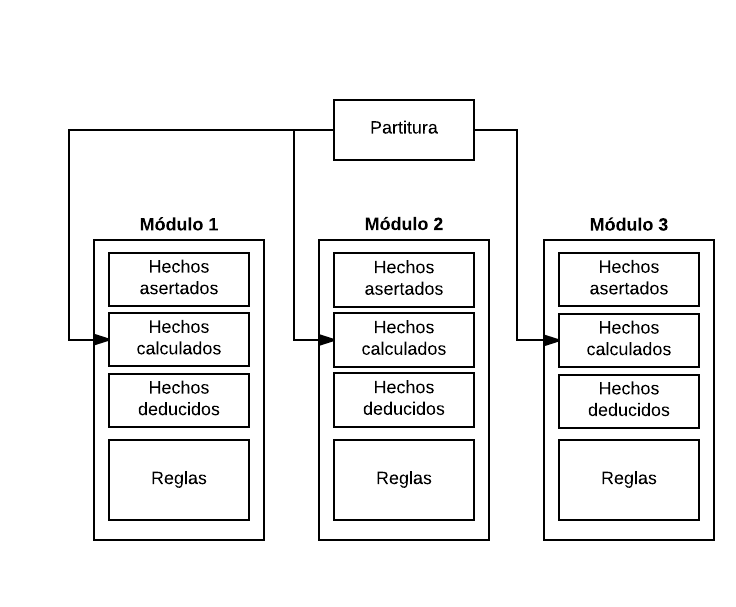
\includegraphics[scale=1]{imagenes/estructuraExp.png}
	\caption{Diagrama de la estructura del sistema experto}
	\label{fig3.1}
\end{figure}